\documentclass[11.5pt]{article}
\usepackage{graphicx} % Required for inserting images
\usepackage{wrapfig}
\usepackage{hyperref}

\title{Git Keeping}
\author{Raisa Nusrat}
\date{September 2023}

\begin{document}

\maketitle

I am a PhD student in Computer Science at UCCS with Dr. Adham Atyabi and my research is on Brain Computer Interface (BCI), particularly human-in-the-loop BCI. This is my first semester working on this area and to start with 
\begin{wrapfigure}{r}{0.25\textwidth} %this figure will be at the right
    \centering
    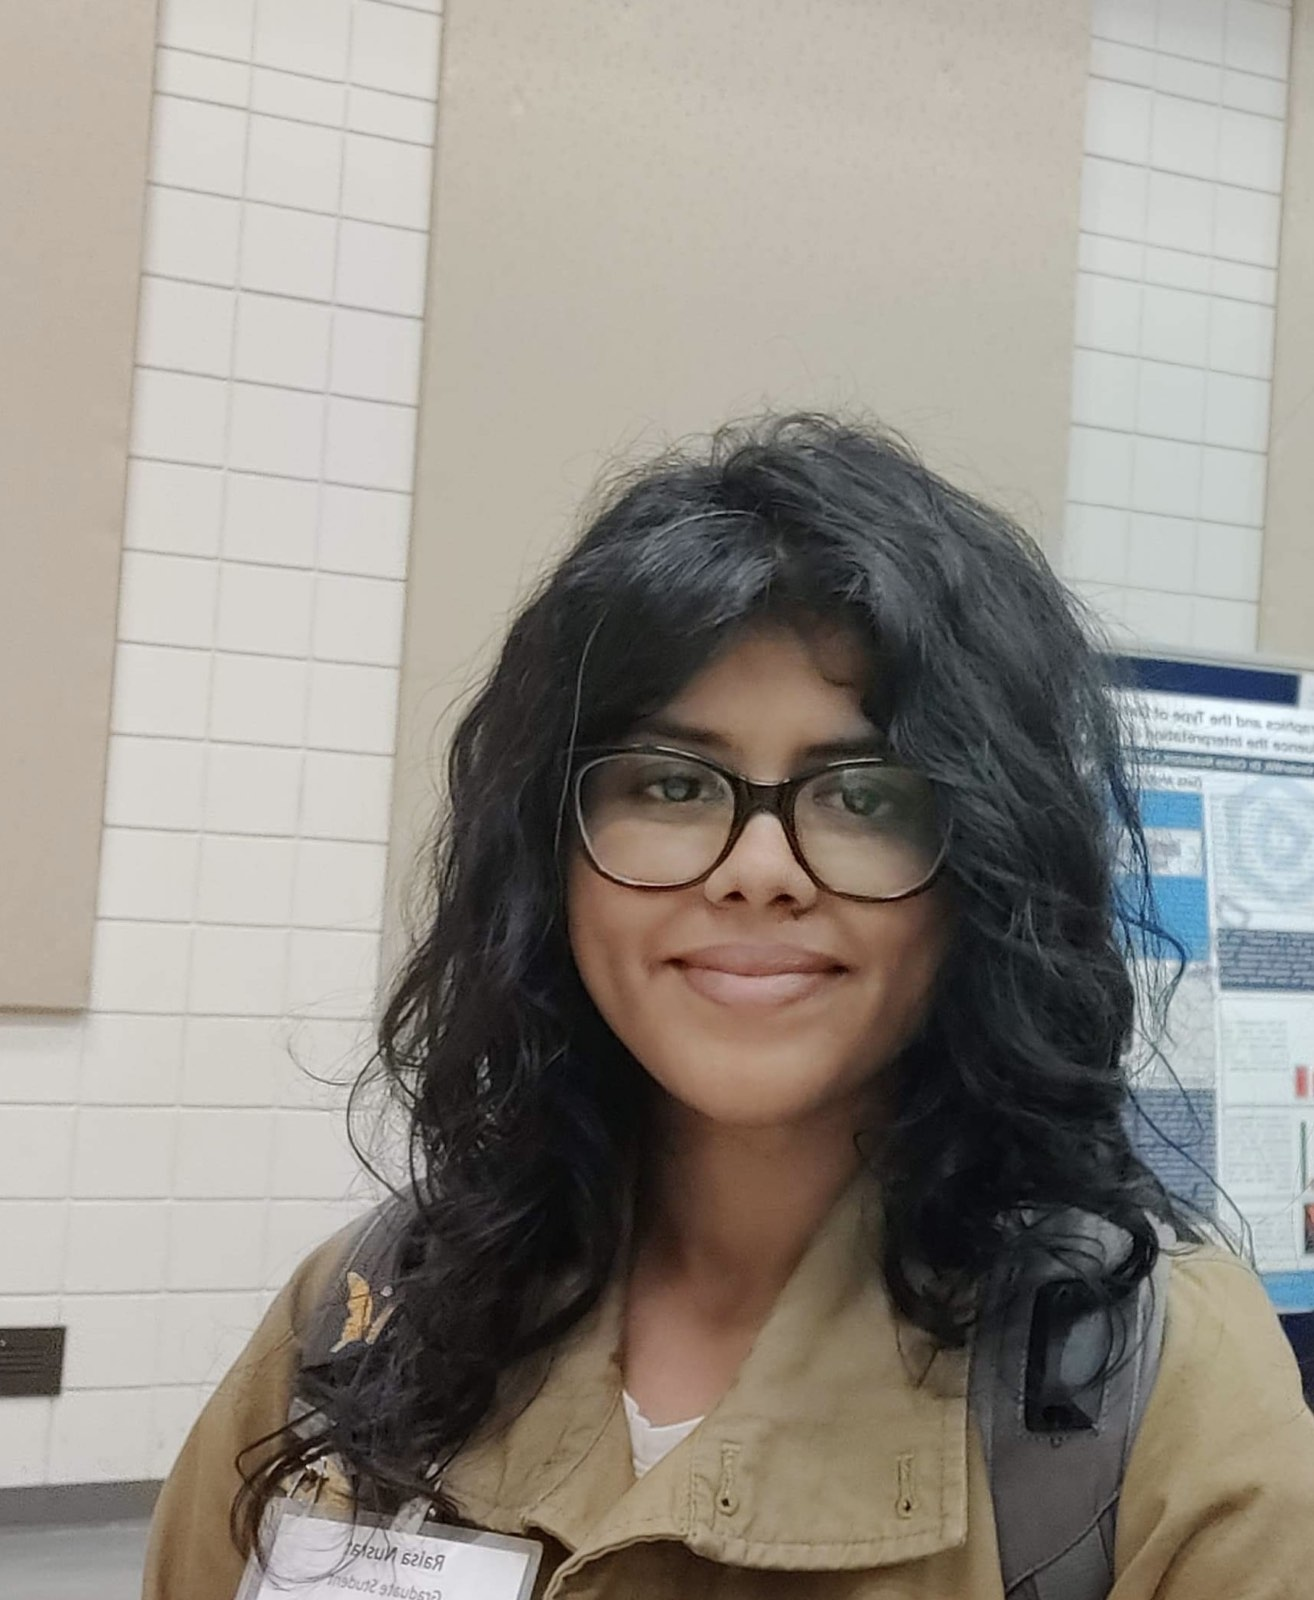
\includegraphics[width=0.25\textwidth]{Raisa_Nusrat.jpg}
\end{wrapfigure}
I need to update myself with advancements in the field, beginning from the history of BCI up until the latest and/ or state of the art methods in BCI. A good way to do so would be to write a review paper on the topic, and here is where I am hoping CS 6000 will serve a dual purpose. Aside from what the course has to offer, I plan to take this opportunity to find and study previously published papers in the area. At the end of the course I hope to have written a review paper on my research area, which I can have published with some evaluation from my mentors. I hope the effect of taking this course will last the lifetime of my academic and professional career. In my personal life, I like to cook, practice being healthful, and learn languages. I used to read fictions a lot when I was younger and I am trying to get back to that again. 
\vspace{.25 cm}

I have been trying to learn about EEG data through and through and how to use Python and MATLAB packages to process and analyze them. Just recently, I used this repository \url{https://github.com/berdakh/mne-codes/blob/main/BCIcompetitionIV2MNE.ipynb} to play around with some EEG data and it was very helpful. The code utilizes MNE which is a python package made for analyzing and visualizing different types of neurophysical data. It is a good alternative for EEGLAB which is MATLAB package for similar purposes.

\end{document}
